\documentclass[border=15pt, tikz]{standalone}
\usepackage[T1]{fontenc}
\usepackage[utf8]{inputenc}
\usepackage{tikz}
\usetikzlibrary{positioning, arrows.meta, decorations.pathreplacing, calc, fit}
\definecolor{clrattention}{HTML}{00B4D8}
\definecolor{clrattention_alt}{HTML}{90E0EF}
\definecolor{clrffn}{HTML}{E63946}
\definecolor{clrnorm}{HTML}{FFBE0B}
\definecolor{clrembed}{HTML}{06D6A0}
\definecolor{clrresidual}{HTML}{118AB2}
\definecolor{clroutput}{HTML}{7B2CBF}
\definecolor{clrspectral}{HTML}{00F5D4}
\definecolor{clrphysics}{HTML}{F77F00}
\definecolor{clrborder}{HTML}{073B4C}
\definecolor{clrtext}{HTML}{073B4C}
\definecolor{clrgroup_frame}{HTML}{073B4C}
\definecolor{clrgroup_fill}{HTML}{EDF6F9}
\begin{document}
\begin{tikzpicture}[
    >=Stealth,
    every node/.style={font=\sffamily},
    block/.style={draw=clrborder, rounded corners=4pt, minimum width=3.8cm,
                  minimum height=0.85cm, font=\sffamily\small\bfseries,
                  text=clrtext, line width=0.6pt},
    arrow/.style={->, thick, color=clrborder, line width=0.7pt, shorten >=1.5pt, shorten <=1.5pt},
    skiparrow/.style={->, thick, color=clrresidual, line width=0.8pt, rounded corners=4pt, shorten >=1.5pt},
    label/.style={font=\sffamily\scriptsize, text=clrtext},
    subtitle/.style={font=\sffamily\footnotesize, text=clrtext},
]
\node[block, fill=clrembed!85, minimum width=3.8cm, minimum height=0.85cm, text=clrtext] (n_1) at (0,0) {Noisy Image};
\node[block, fill=clrattention!85, minimum width=7.0cm, minimum height=0.85cm, text=clrtext, right=0.4cm of n_1] (n_2) {Patchify 4x4};
\node[circle, draw=clrborder, fill=clrresidual!30, inner sep=2pt, font=\sffamily\scriptsize\bfseries, right=0.3cm of n_2] (n_3) {Pos. Embedding};
\node[block, fill=clrresidual!85, minimum width=3.8cm, minimum height=0.85cm, text=clrtext, right=0.4cm of n_3] (n_4) {Timestep + Class Emb};
\node[block, fill=clrnorm!85, minimum width=3.4cm, minimum height=0.65cm, text=clrtext, right=0.4cm of n_4] (n_5) {AdaLN};
\node[inner sep=0, minimum size=0, right=0.4cm of n_5] (res_entry_6) {};
\node[block, fill=clrnorm!85, minimum width=3.8cm, minimum height=0.85cm, text=clrtext, right=0.4cm of res_entry_6] (n_7) {LayerNorm};
\node[block, fill=clrattention_alt!85, minimum width=3.8cm, minimum height=0.85cm, text=clrtext, right=0.4cm of n_7] (n_8) {Self-Attention};
\node[circle, draw=clrborder, fill=clrresidual!30, inner sep=2pt, font=\sffamily\scriptsize\bfseries, right=0.3cm of n_8] (add_9) {+};
\node[inner sep=0, minimum size=0, right=0.4cm of add_9] (res_entry_10) {};
\node[block, fill=clrnorm!85, minimum width=3.8cm, minimum height=0.85cm, text=clrtext, right=0.4cm of res_entry_10] (n_11) {LayerNorm};
\node[block, fill=clrffn!85, minimum width=3.8cm, minimum height=0.85cm, text=clrtext, right=0.4cm of n_11] (n_12) {FFN (GeLU)};
\node[circle, draw=clrborder, fill=clrresidual!30, inner sep=2pt, font=\sffamily\scriptsize\bfseries, right=0.3cm of n_12] (add_13) {+};
\node[block, fill=clrnorm!85, minimum width=3.4cm, minimum height=0.65cm, text=clrtext, right=0.4cm of add_13] (n_14) {AdaLN};
\node[inner sep=0, minimum size=0, right=0.4cm of n_14] (res_entry_15) {};
\node[block, fill=clrnorm!85, minimum width=3.8cm, minimum height=0.85cm, text=clrtext, right=0.4cm of res_entry_15] (n_16) {LayerNorm};
\node[block, fill=clrattention_alt!85, minimum width=3.8cm, minimum height=0.85cm, text=clrtext, right=0.4cm of n_16] (n_17) {Self-Attention};
\node[circle, draw=clrborder, fill=clrresidual!30, inner sep=2pt, font=\sffamily\scriptsize\bfseries, right=0.3cm of n_17] (add_18) {+};
\node[inner sep=0, minimum size=0, right=0.4cm of add_18] (res_entry_19) {};
\node[block, fill=clrnorm!85, minimum width=3.8cm, minimum height=0.85cm, text=clrtext, right=0.4cm of res_entry_19] (n_20) {LayerNorm};
\node[block, fill=clrffn!85, minimum width=3.8cm, minimum height=0.85cm, text=clrtext, right=0.4cm of n_20] (n_21) {FFN (GeLU)};
\node[circle, draw=clrborder, fill=clrresidual!30, inner sep=2pt, font=\sffamily\scriptsize\bfseries, right=0.3cm of n_21] (add_22) {+};
\node[block, fill=clrresidual!85, minimum width=2.0cm, minimum height=1.0cm, text=clrtext, right=0.4cm of add_22] (n_23) {Linear Decoder};
\node[block, fill=clrattention_alt!85, minimum width=3.8cm, minimum height=0.85cm, text=clrtext, right=0.4cm of n_23] (n_24) {De-patchify};
\node[block, fill=clrphysics!85, minimum width=3.0cm, minimum height=0.85cm, text=clrtext, right=0.4cm of n_24] (n_25) {Noise Prediction};
\draw[arrow] (n_1.east) -- (n_2.west);
\draw[arrow] (n_2.east) -- (n_3.west);
\draw[arrow] (n_3.east) -- (n_4.west);
\draw[arrow] (n_4.east) -- (n_5.west);
\draw[arrow] (n_7.east) -- (n_8.west);
\draw[arrow] (res_entry_6.east) -- (n_7.west);
\draw[arrow] (n_8.east) -- (add_9.west);
\draw[skiparrow] (res_entry_6.east) -- ++(2.4,0) |- (add_9.east);
\draw[arrow] (n_11.east) -- (n_12.west);
\draw[arrow] (res_entry_10.east) -- (n_11.west);
\draw[arrow] (n_12.east) -- (add_13.west);
\draw[skiparrow] (res_entry_10.east) -- ++(2.4,0) |- (add_13.east);
\draw[arrow] (add_9.east) -- (res_entry_10.west);
\draw[arrow] (n_5.east) -- (res_entry_6.west);
\draw[arrow] (add_13.east) -- (n_14.west);
\draw[arrow] (n_16.east) -- (n_17.west);
\draw[arrow] (res_entry_15.east) -- (n_16.west);
\draw[arrow] (n_17.east) -- (add_18.west);
\draw[skiparrow] (res_entry_15.east) -- ++(2.4,0) |- (add_18.east);
\draw[arrow] (n_20.east) -- (n_21.west);
\draw[arrow] (res_entry_19.east) -- (n_20.west);
\draw[arrow] (n_21.east) -- (add_22.west);
\draw[skiparrow] (res_entry_19.east) -- ++(2.4,0) |- (add_22.east);
\draw[arrow] (add_18.east) -- (res_entry_19.west);
\draw[arrow] (n_14.east) -- (res_entry_15.west);
\draw[arrow] (add_22.east) -- (n_23.west);
\draw[arrow] (n_23.east) -- (n_24.west);
\draw[arrow] (n_24.east) -- (n_25.west);
\draw[arrow] ([xshift=-0.6cm]n_1.west) -- node[right, yshift=-2pt, font=\sffamily\scriptsize, text=clrtext] {Input} (n_1.west);
\draw[arrow] (n_25.east) -- node[right, yshift=-2pt, font=\sffamily\scriptsize, text=clrtext] {Output} ([xshift=0.6cm]n_25.east);
\node[draw=clrgroup_frame!60, rounded corners=8pt, densely dashed, line width=0.6pt, fill=clrgroup_fill, fill opacity=0.35, inner ysep=0.55cm, inner xsep=0.7cm, fit=(n_5) (n_7) (n_8) (n_11) (n_12) (n_14) (n_16) (n_17) (n_20) (n_21)] (g_0) {};
\node[below=10pt of g_0.south, anchor=north, font=\sffamily\Large\bfseries, text=clrborder] (g_0_badge) {$\times12$};
\node[below=0.6cm of current bounding box.south, subtitle, text width=14cm, align=center] {\textbf{DiT-B/4 -- Diffusion Transformer}};
\end{tikzpicture}
\end{document}
